\documentclass{article}\usepackage[]{graphicx}\usepackage[]{xcolor}
% maxwidth is the original width if it is less than linewidth
% otherwise use linewidth (to make sure the graphics do not exceed the margin)
\makeatletter
\def\maxwidth{ %
  \ifdim\Gin@nat@width>\linewidth
    \linewidth
  \else
    \Gin@nat@width
  \fi
}
\makeatother

\definecolor{fgcolor}{rgb}{0.345, 0.345, 0.345}
\newcommand{\hlnum}[1]{\textcolor[rgb]{0.686,0.059,0.569}{#1}}%
\newcommand{\hlsng}[1]{\textcolor[rgb]{0.192,0.494,0.8}{#1}}%
\newcommand{\hlcom}[1]{\textcolor[rgb]{0.678,0.584,0.686}{\textit{#1}}}%
\newcommand{\hlopt}[1]{\textcolor[rgb]{0,0,0}{#1}}%
\newcommand{\hldef}[1]{\textcolor[rgb]{0.345,0.345,0.345}{#1}}%
\newcommand{\hlkwa}[1]{\textcolor[rgb]{0.161,0.373,0.58}{\textbf{#1}}}%
\newcommand{\hlkwb}[1]{\textcolor[rgb]{0.69,0.353,0.396}{#1}}%
\newcommand{\hlkwc}[1]{\textcolor[rgb]{0.333,0.667,0.333}{#1}}%
\newcommand{\hlkwd}[1]{\textcolor[rgb]{0.737,0.353,0.396}{\textbf{#1}}}%
\let\hlipl\hlkwb

\usepackage{framed}
\makeatletter
\newenvironment{kframe}{%
 \def\at@end@of@kframe{}%
 \ifinner\ifhmode%
  \def\at@end@of@kframe{\end{minipage}}%
  \begin{minipage}{\columnwidth}%
 \fi\fi%
 \def\FrameCommand##1{\hskip\@totalleftmargin \hskip-\fboxsep
 \colorbox{shadecolor}{##1}\hskip-\fboxsep
     % There is no \\@totalrightmargin, so:
     \hskip-\linewidth \hskip-\@totalleftmargin \hskip\columnwidth}%
 \MakeFramed {\advance\hsize-\width
   \@totalleftmargin\z@ \linewidth\hsize
   \@setminipage}}%
 {\par\unskip\endMakeFramed%
 \at@end@of@kframe}
\makeatother

\definecolor{shadecolor}{rgb}{.97, .97, .97}
\definecolor{messagecolor}{rgb}{0, 0, 0}
\definecolor{warningcolor}{rgb}{1, 0, 1}
\definecolor{errorcolor}{rgb}{1, 0, 0}
\newenvironment{knitrout}{}{} % an empty environment to be redefined in TeX

\usepackage{alltt}
\usepackage[margin=1.0in]{geometry} % To set margins
\usepackage{amsmath}  % This allows me to use the align functionality.
                      % If you find yourself trying to replicate
                      % something you found online, ensure you're
                      % loading the necessary packages!
\usepackage{amsfonts} % Math font
\usepackage{fancyvrb}
\usepackage{hyperref} % For including hyperlinks
\usepackage[shortlabels]{enumitem}% For enumerated lists with labels specified
                                  % We had to run tlmgr_install("enumitem") in R
\usepackage{float}    % For telling R where to put a table/figure
\usepackage{natbib}        %For the bibliography
\bibliographystyle{apalike}%For the bibliography
\IfFileExists{upquote.sty}{\usepackage{upquote}}{}
\begin{document}

In lecture 16, we looked at precipitation amounts in Madison County (at 
Morrisville station). We found that the Weibull distribution had a good fit
to the monthly precipitation amounts.\\

We found that the MLEs for the Weibull distribution were 
\begin{align*}
    \hat{a}&=2.1871\\
    \hat{\sigma}&=3.9683
\end{align*}
and
\[-\mathcal{L}(\{\hat{a}, \hat{\sigma}\}|\mathbf{x}) = 2166.496\]
is the realized negative log-likelihood.
Note this means that the log-likelihood is
\[\mathcal{L}(\{\hat{a}, \hat{\sigma}\}|\mathbf{x}) = -2166.496,\]
and the usual likelihood is
\[L(\{\hat{a}, \hat{\sigma}\}|\mathbf{x}) = e^{\left[\mathcal{L}(\{\hat{a}, \hat{\sigma}\}|\mathbf{x})\right]} \approx = e^{-2166.496},\]
which \texttt{R} cannot differentiate from 0.

\begin{enumerate}
  \item Someone asked ``why Weibull?" in class. That is, why wouldn't we use 
  another right-skewed distribution like the Gamma (see Lecture 15), or
  the Log-Normal (see Lecture 17).
  
\begin{knitrout}\scriptsize
\definecolor{shadecolor}{rgb}{0.969, 0.969, 0.969}\color{fgcolor}\begin{kframe}
\begin{alltt}
\hlcom{# Load and clean data about precipitation in Madison County}
\hldef{dat.precip} \hlkwb{<-} \hlkwd{read_csv}\hldef{(}\hlkwc{file} \hldef{=} \hlsng{"agacis.csv"}\hldef{)}

\hldef{dat.precip.long} \hlkwb{<-} \hldef{dat.precip |>}
\hldef{dplyr}\hlopt{::}\hlkwd{select}\hldef{(}\hlopt{-}\hldef{Annual) |>}                   \hlcom{# Remove annual column }
\hlkwd{pivot_longer}\hldef{(}\hlkwc{cols} \hldef{=} \hlkwd{c}\hldef{(Jan, Feb, Mar, Apr,}   \hlcom{# pivot the column data into one col}
                      \hldef{May, Jun, Jul, Aug,}
                      \hldef{Sep, Oct, Nov, Dec),}
             \hlkwc{values_to} \hldef{=} \hlsng{"Precipitation"}\hldef{,}   \hlcom{# store the values in Precipitation}
             \hlkwc{names_to} \hldef{=} \hlsng{"Month"}\hldef{) |>}         \hlcom{# store the months in Month}
\hlcom{#switch 'M' to NA values and convert numbers to integers from Strings}
\hlkwd{mutate}\hldef{(}\hlkwc{Precipitation} \hldef{=} \hlkwd{case_when}\hldef{(Precipitation} \hlopt{==} \hlsng{"M"} \hlopt{~} \hlnum{NA_character_}\hldef{,}
                                 \hlnum{TRUE}                 \hlopt{~} \hldef{Precipitation))|>}
\hlkwd{mutate}\hldef{(}\hlkwc{Precipitation} \hldef{=} \hlkwd{as.numeric}\hldef{(Precipitation))}
\end{alltt}
\end{kframe}
\end{knitrout}
\begin{enumerate}
    \item Compute the MLEs for these data using a Gamma distribution.
\begin{knitrout}\scriptsize
\definecolor{shadecolor}{rgb}{0.969, 0.969, 0.969}\color{fgcolor}\begin{kframe}
\begin{alltt}
\hlcom{#Function to compute Maximum Likelihood}
\hldef{llgamma} \hlkwb{<-} \hlkwa{function}\hldef{(}\hlkwc{par}\hldef{,} \hlkwc{data}\hldef{,} \hlkwc{neg} \hldef{= F)\{}
  \hldef{alpha} \hlkwb{<-} \hldef{par[}\hlnum{1}\hldef{]} \hlcom{#get alpha and beta}
  \hldef{beta} \hlkwb{<-} \hldef{par[}\hlnum{2}\hldef{]}

  \hlcom{#compute log likelihood}
  \hldef{loglik} \hlkwb{<-} \hlkwd{sum}\hldef{(}\hlkwd{log}\hldef{(}\hlkwd{dgamma}\hldef{(}\hlkwc{x} \hldef{= data,} \hlkwc{shape} \hldef{= alpha,} \hlkwc{rate} \hldef{= beta)),} \hlkwc{na.rm} \hldef{= T)}

  \hlkwd{return}\hldef{(}\hlkwd{ifelse}\hldef{(neg,} \hlopt{-} \hldef{loglik, loglik))}
\hldef{\}}

\hlcom{#Compute MLE }
\hldef{MLE.gamma} \hlkwb{<-} \hlkwd{optim}\hldef{(}\hlkwc{par} \hldef{=} \hlkwd{c}\hldef{(}\hlnum{1}\hldef{,}\hlnum{1}\hldef{),}
               \hlkwc{fn} \hldef{= llgamma,}
               \hlkwc{data}\hldef{=dat.precip.long}\hlopt{$}\hldef{Precipitation,}
               \hlkwc{neg}\hldef{=T)}

\hlcom{#extract alpha and beta}
\hldef{alpha.MLE} \hlkwb{<-} \hldef{MLE.gamma}\hlopt{$}\hldef{par[}\hlnum{1}\hldef{]}
\hldef{beta.MLE} \hlkwb{<-} \hldef{MLE.gamma}\hlopt{$}\hldef{par[}\hlnum{2}\hldef{]}

\hlcom{#print the values}
\hldef{alpha.MLE}
\end{alltt}
\begin{verbatim}
## [1] 4.174581
\end{verbatim}
\begin{alltt}
\hldef{beta.MLE}
\end{alltt}
\begin{verbatim}
## [1] 1.189099
\end{verbatim}
\end{kframe}
\end{knitrout}
We computed the MLEs for these data using a Gamma distribution to obtain $\alpha = 4.1745814$ and $\beta = 1.1890993$.
    \item Compute the MLEs for these data using the Log-Normal distribution.
\begin{knitrout}\scriptsize
\definecolor{shadecolor}{rgb}{0.969, 0.969, 0.969}\color{fgcolor}\begin{kframe}
\begin{alltt}
\hlcom{#Function to compute Maximum Likelihood}
\hldef{lllognorm} \hlkwb{<-} \hlkwa{function}\hldef{(}\hlkwc{par}\hldef{,} \hlkwc{data}\hldef{,} \hlkwc{neg} \hldef{= F)\{}
  \hldef{mu} \hlkwb{<-} \hldef{par[}\hlnum{1}\hldef{]} \hlcom{#get mu and sigma}
  \hldef{sigma} \hlkwb{<-} \hldef{par[}\hlnum{2}\hldef{]}

  \hlcom{#compute log likelihood}
  \hldef{loglik} \hlkwb{<-} \hlkwd{sum}\hldef{(}\hlkwd{log}\hldef{(}\hlkwd{dlnorm}\hldef{(}\hlkwc{x} \hldef{= data,} \hlkwc{meanlog} \hldef{= mu,} \hlkwc{sdlog} \hldef{= sigma)),} \hlkwc{na.rm} \hldef{= T)}

  \hlkwd{return}\hldef{(}\hlkwd{ifelse}\hldef{(neg,} \hlopt{-} \hldef{loglik, loglik))}
\hldef{\}}

\hlcom{#Compute MLE }
\hldef{MLE.lognorm} \hlkwb{<-} \hlkwd{optim}\hldef{(}\hlkwc{par} \hldef{=} \hlkwd{c}\hldef{(}\hlnum{1}\hldef{,}\hlnum{1}\hldef{),}
               \hlkwc{fn} \hldef{= lllognorm,}
               \hlkwc{data}\hldef{=dat.precip.long}\hlopt{$}\hldef{Precipitation,}
               \hlkwc{neg}\hldef{=T)}

\hlcom{#extract alpha and beta}
\hldef{mu.MLE} \hlkwb{<-} \hldef{MLE.lognorm}\hlopt{$}\hldef{par[}\hlnum{1}\hldef{]}
\hldef{sigma.MLE} \hlkwb{<-} \hldef{MLE.lognorm}\hlopt{$}\hldef{par[}\hlnum{2}\hldef{]}

\hlcom{#print the values}
\hldef{mu.MLE}
\end{alltt}
\begin{verbatim}
## [1] 1.131261
\end{verbatim}
\begin{alltt}
\hldef{sigma.MLE}
\end{alltt}
\begin{verbatim}
## [1] 0.5333417
\end{verbatim}
\end{kframe}
\end{knitrout}
We computed the MLEs for these data using a Log-Normal distribution to obtain $\mu = 1.1312609$ and $\sigma = 0.5333417$.
    \item Compute the likelihood ratio to compare the Weibull and the Gamma distribution. 
    Which has a better fit according to the likelhiood ratio?
    \[Q = \frac{L(\{\hat{a}, \hat{\sigma}\}|\mathbf{x})}{L(\{\hat{\alpha}, \hat{\beta}\}|\mathbf{x})}=e^{\left[\mathcal{L}(\{\hat{a}, \hat{\sigma}\}|\mathbf{x}) - \mathcal{L}(\{\hat{\alpha}, \hat{\beta}\}|\mathbf{x})\right]}\]
\begin{knitrout}\scriptsize
\definecolor{shadecolor}{rgb}{0.969, 0.969, 0.969}\color{fgcolor}\begin{kframe}
\begin{alltt}
\hlcom{#compute log-likelihood for Gamma distribution}
\hldef{Gamma.loglik} \hlkwb{<-} \hlkwd{llgamma}\hldef{(}\hlkwc{par} \hldef{=} \hlkwd{c}\hldef{(alpha.MLE, beta.MLE),} \hlkwc{data} \hldef{= dat.precip.long}\hlopt{$}\hldef{Precipitation,} \hlkwc{neg} \hldef{= F)}

\hlcom{#compute the likelihood ratio}
\hldef{Weibull.loglik} \hlkwb{<-} \hlopt{-}\hlnum{2166.496}
\hldef{q.gamma.weibull} \hlkwb{<-} \hlkwd{exp}\hldef{(Weibull.loglik}\hlopt{-}\hldef{Gamma.loglik)}

\hlcom{#print Q}
\hldef{q.gamma.weibull}
\end{alltt}
\begin{verbatim}
## [1] 2.161318e-07
\end{verbatim}
\end{kframe}
\end{knitrout}
The likelihood ratio of the Weibull and the Gamma distribution is \ensuremath{2.1613179\times 10^{-7}}. Because $Q < 1$ , the Gamma distribution is a better fit according to the likelihood ratio. 
    \item Compute the likelihood ratio to compare the Weibull and the Log-Normal distribution.
    Which has a better fit according to the likelihood ratio?
    \[Q = \frac{L(\{\hat{a}, \hat{\sigma}\}|\mathbf{x})}{L(\{\hat{\mu}, \hat{\sigma}\}|\mathbf{x})}=e^{\left[\mathcal{L}(\{\hat{a}, \hat{\sigma}\}|\mathbf{x}) - \mathcal{L}(\{\hat{\mu}, \hat{\sigma}\}|\mathbf{x})\right]}\]
\begin{knitrout}\scriptsize
\definecolor{shadecolor}{rgb}{0.969, 0.969, 0.969}\color{fgcolor}\begin{kframe}
\begin{alltt}
\hlcom{#compute log-likelihood for Log-Normal distribution}
\hldef{Lognorm.loglik} \hlkwb{<-} \hlkwd{lllognorm}\hldef{(}\hlkwd{c}\hldef{(mu.MLE, sigma.MLE),} \hlkwc{data} \hldef{= dat.precip.long}\hlopt{$}\hldef{Precipitation,} \hlkwc{neg} \hldef{= F)}

\hlcom{#compute the likelihood ratio}
\hldef{q.lognorm.weibull} \hlkwb{<-} \hlkwd{exp}\hldef{(Weibull.loglik}\hlopt{-}\hldef{Lognorm.loglik)}

\hlcom{#print Q}
\hldef{q.lognorm.weibull}
\end{alltt}
\begin{verbatim}
## [1] 2.370668e+16
\end{verbatim}
\end{kframe}
\end{knitrout}
The likelihood ratio of the Weibull and the Log-Normal distribution is \ensuremath{2.3706676\times 10^{16}}. Because $Q > 1$ , the Weibull distribution it is a better fit according to the likelihood ratio. 

    \item Compute the likelihood ratio to compare the Gamma and the Log-Normal distribution.
    Which has a better fit according to the likelhiood ratio?
    \[Q = \frac{L(\{\hat{\alpha}, \hat{\beta}\}|\mathbf{x})}{L(\{\hat{\mu}, \hat{\sigma}\}|\mathbf{x})}=e^{\left[\mathcal{L}(\{\hat{\alpha}, \hat{\beta}\}|\mathbf{x}) - \mathcal{L}(\{\hat{\mu}, \hat{\sigma}\}|\mathbf{x})\right]}\]
\begin{knitrout}\scriptsize
\definecolor{shadecolor}{rgb}{0.969, 0.969, 0.969}\color{fgcolor}\begin{kframe}
\begin{alltt}
\hlcom{#compute the likelihood ratio}
\hldef{q.gamma.lognorm} \hlkwb{<-} \hlkwd{exp}\hldef{(Gamma.loglik}\hlopt{-}\hldef{Lognorm.loglik)}

\hlcom{#print Q}
\hldef{q.gamma.lognorm}
\end{alltt}
\begin{verbatim}
## [1] 1.096862e+23
\end{verbatim}
\end{kframe}
\end{knitrout}
The likelihood ratio of the Gamma and the Log-Normal distribution is \ensuremath{1.096862\times 10^{23}}. Because $Q > 1$, the Gamma distribution is a better fit according to the likelihood ratio. 
  \end{enumerate}

\end{enumerate}

\begin{figure}
 \centering
 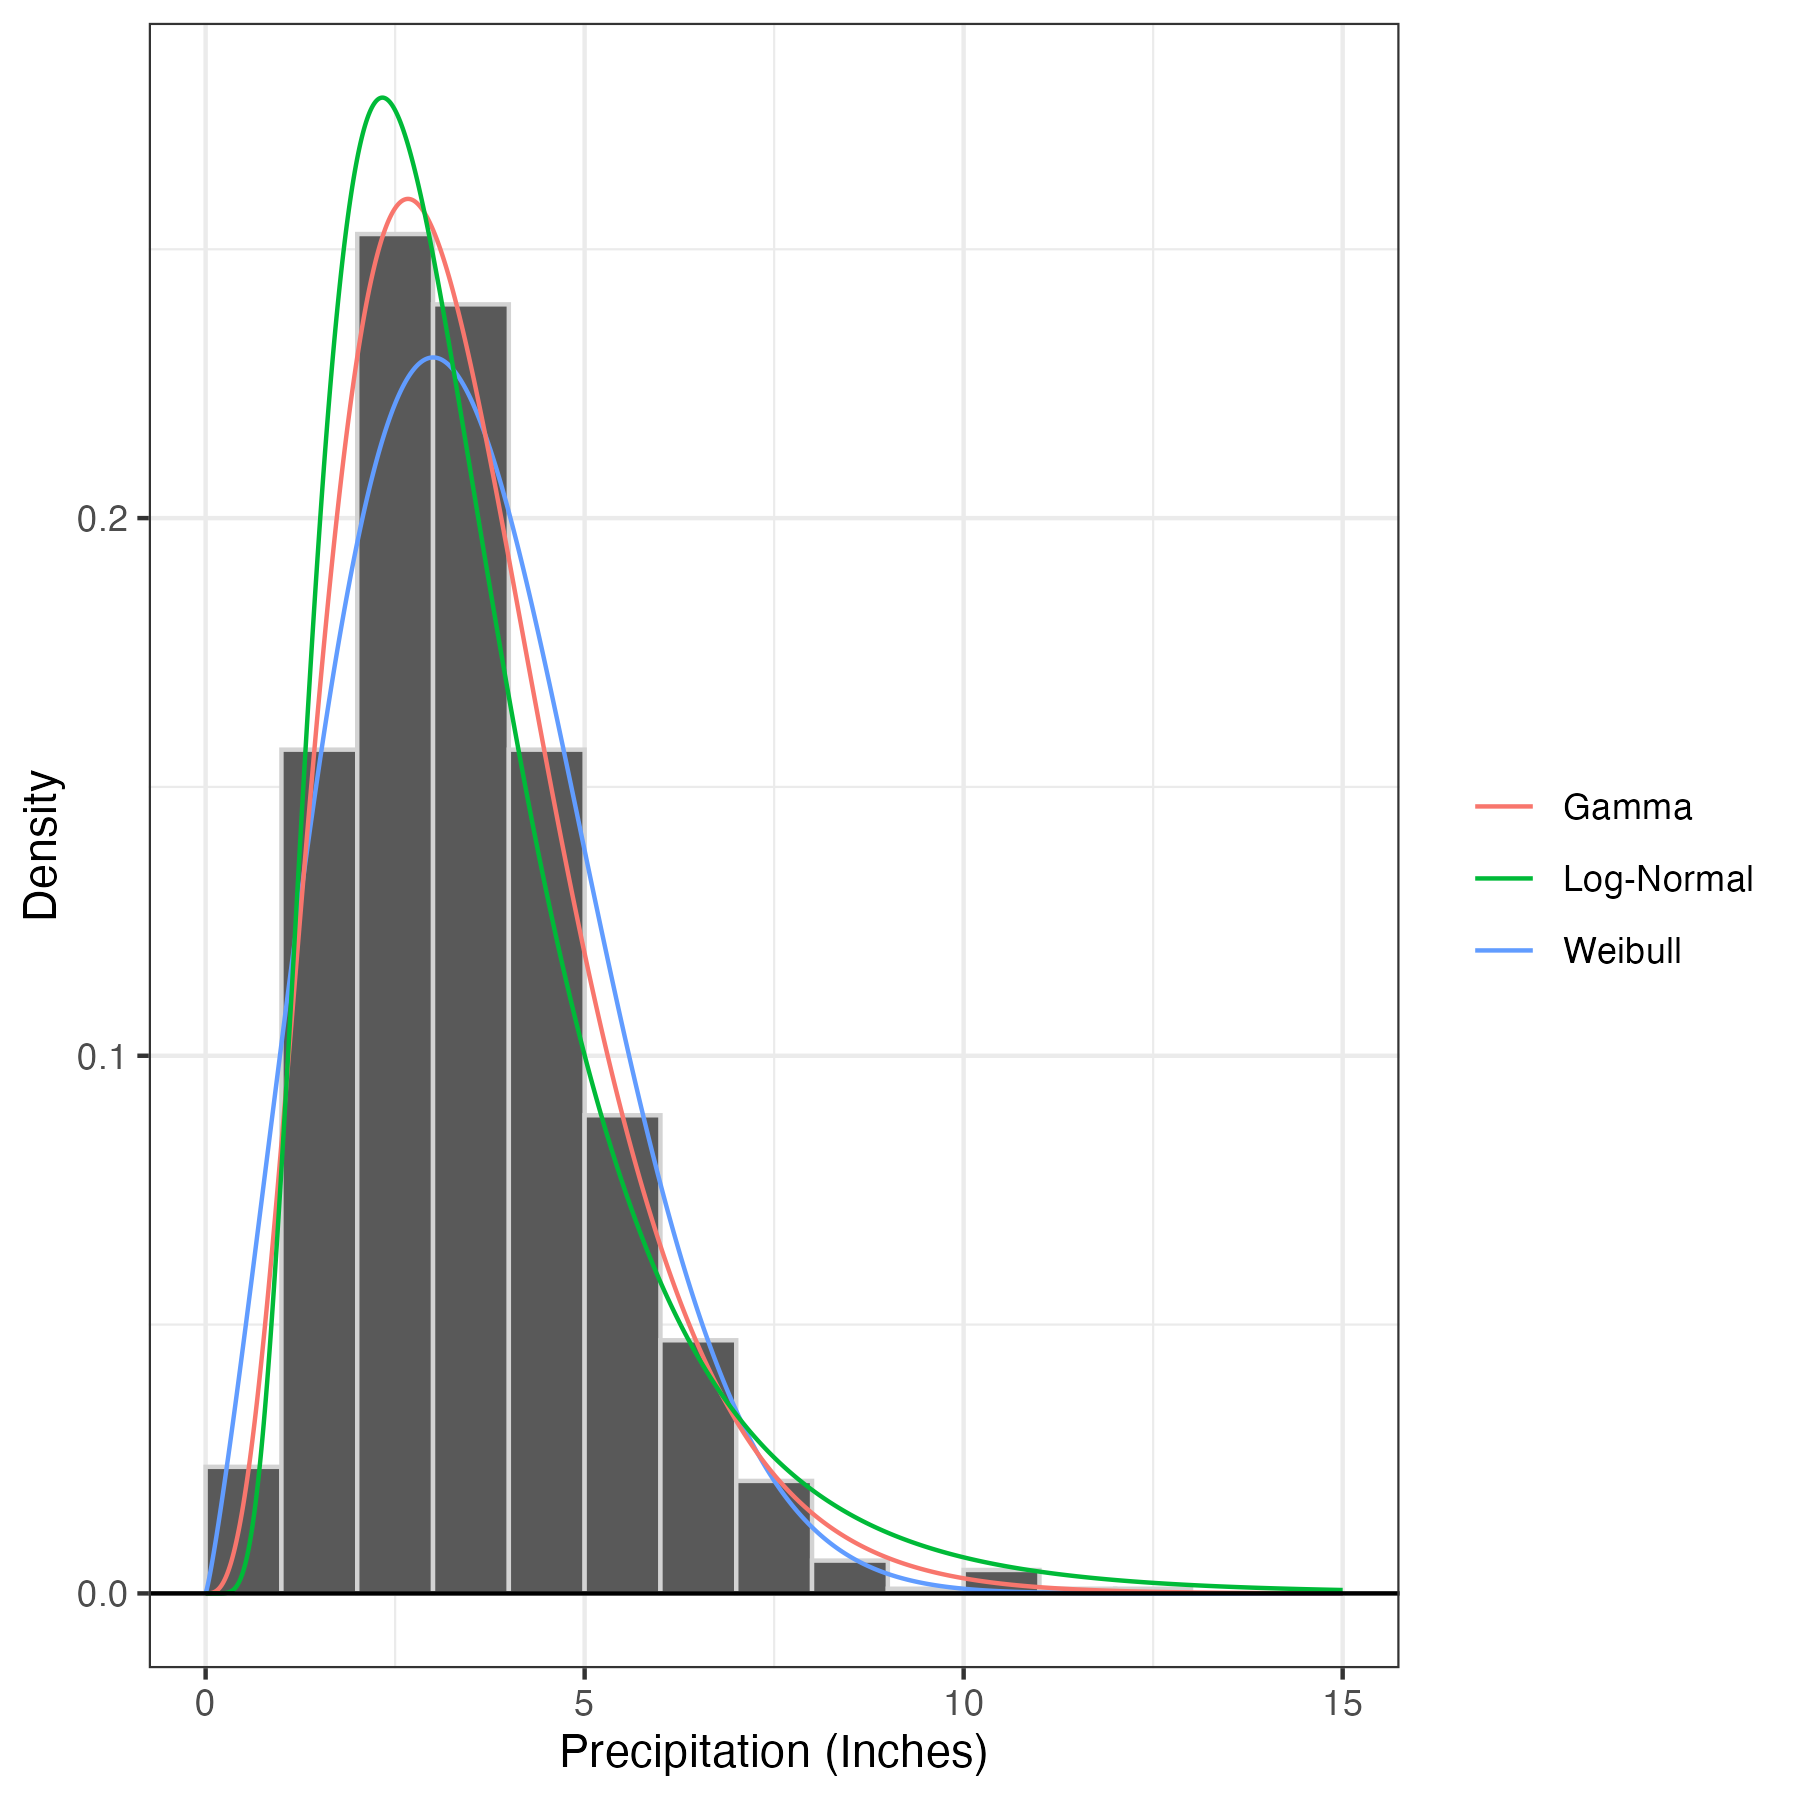
\includegraphics[width=0.5\textwidth]{histogram.png}
 \caption{Superimposed distributions onto the percipitation data}
 \label{fig:label}
\end{figure}

\bibliography{bibliography}
\end{document}
